\documentclass[aspectratio=169]{beamer}

\usetheme{Madrid}
\usecolortheme{seahorse}
\usepackage{booktabs}
\usepackage{graphicx}
\usepackage{listings}
\usepackage{tikz}
\usepackage{xcolor}

% Custom colours
\definecolor{leafgreen}{RGB}{34,139,34}
\definecolor{diseasered}{RGB}{180,40,40}
\definecolor{codegray}{RGB}{245,245,245}

\lstset{
  basicstyle=\ttfamily\scriptsize,
  backgroundcolor=\color{codegray},
  frame=single,
  breaklines=true,
}

\title[Edge AI Plant Disease Detection]{\textbf{Edge AI Plant Disease Detection System}}
\subtitle{Real-Time Offline Inference on Raspberry Pi 5}
\author{Aayush Jeevan Patil (22220) \and Vansh Dhar (22156)}
\institute{Edge AI Course}
\date{May 2026}

% Progress bar at bottom
\setbeamertemplate{footline}[frame number]
\setbeamertemplate{navigation symbols}{}

% ─────────────────────────────────────────────────────────────────────────────
\begin{document}

\begin{frame}
  \titlepage
\end{frame}

% ─────────────────────────────────────────────────────────────────────────────
\begin{frame}{Outline}
  \tableofcontents
\end{frame}

% ─────────────────────────────────────────────────────────────────────────────
\section{Problem \& Motivation}

\begin{frame}{Problem \& Motivation}
  \begin{columns}
    \column{0.55\textwidth}
      \textbf{Problem}
      \begin{itemize}
        \item Farmers lack timely access to agricultural experts
        \item Undetected crop diseases $\Rightarrow$ yield losses
        \item Existing solutions require internet, lab equipment, or trained staff
      \end{itemize}
      \vspace{0.4cm}
      \textbf{Why Edge AI?}
      \begin{itemize}
        \item \textcolor{leafgreen}{\textbf{No connectivity}} needed in the field
        \item \textcolor{leafgreen}{\textbf{Instant}} — no cloud round-trip latency
        \item \textcolor{leafgreen}{\textbf{Privacy}} — images stay on device
        \item \textcolor{leafgreen}{\textbf{Low cost}} — runs on a \$80 Raspberry Pi
      \end{itemize}
    \column{0.42\textwidth}
      \begin{block}{Goal}
        A farmer holds a leaf in front of a camera and instantly sees the disease name and confidence score — \textbf{offline, in real time}.
      \end{block}
      \vspace{0.3cm}
      \textbf{Target metrics}
      \begin{itemize}
        \item Inference $<$ 1.5 s per frame
        \item Model file $<$ 10 MB
        \item Val accuracy $\geq$ 85\%
      \end{itemize}
  \end{columns}
\end{frame}

% ─────────────────────────────────────────────────────────────────────────────
\section{Dataset}

\begin{frame}{Dataset — PlantVillage}
  \begin{columns}
    \column{0.48\textwidth}
      \textbf{Source:} PlantVillage (color variant)\\
      \small\url{kaggle.com/datasets/emmarex/plantdisease}\\[0.3cm]
      \textbf{Full dataset:} 38 classes, $\sim$54,000 images\\[0.3cm]
      \textbf{Four dataset modes implemented:}
      \begin{center}
      \begin{tabular}{ll}
        \toprule
        Mode & Classes \\
        \midrule
        \texttt{tomato\_5}   & 5  \\
        \texttt{tomato\_10}  & 10 \\
        \texttt{multi\_crop} & 15 \\
        \texttt{balanced}    & \textbf{15} \\
        \bottomrule
      \end{tabular}
      \end{center}
    \column{0.48\textwidth}
      \textbf{Final mode: \texttt{balanced}}
      \begin{itemize}
        \item Tomato $\times$ 10 (all diseases)
        \item Potato $\times$ 3
        \item Pepper $\times$ 2
        \item \textbf{Hard cap: 1,000 images/class}
      \end{itemize}
      \vspace{0.2cm}
      \begin{alertblock}{Why the cap?}
        PlantVillage ranges from 152 (Potato healthy) to 5,357 (Tomato YLCV) images. Without capping, the model collapsed to always predicting the majority class.
      \end{alertblock}
  \end{columns}
\end{frame}

\begin{frame}{Dataset — Preprocessing \& Augmentation}
  \begin{columns}
    \column{0.48\textwidth}
      \textbf{Preprocessing}
      \begin{itemize}
        \item Resize $\rightarrow$ 224$\times$224 (Lanczos)
        \item Convert to RGB
        \item Stratified split: \textbf{70 / 15 / 15}\\
              train / val / test, seed = 42
        \item Zero data leakage verified\\
              (all pairwise split intersections empty)
        \item Labels written to \texttt{models/labels.txt}
      \end{itemize}
    \column{0.48\textwidth}
      \textbf{Augmentation} (training split only)
      \begin{center}
      \begin{tabular}{ll}
        \toprule
        Transform & Params \\
        \midrule
        H-flip        & p = 0.5 \\
        V-flip        & p = 0.5 \\
        Rotation      & $\pm$30° \\
        Resized crop  & 90–100\% \\
        Colour jitter & bright $\pm$0.2, \\
                      & contrast $\pm$0.3 \\
        ImageNet norm & $\mu$=[.485,.456,.406] \\
        \bottomrule
      \end{tabular}
      \end{center}
  \end{columns}
\end{frame}

% ─────────────────────────────────────────────────────────────────────────────
\section{Model Architecture \& Training}

\begin{frame}{Model — MobileNetV3-Small}
  \begin{columns}
    \column{0.55\textwidth}
      \textbf{Why MobileNetV3-Small?}
      \begin{itemize}
        \item Only \textbf{56 MFLOPs/image} — fits ARM CPU budget
        \item ImageNet pretrained $\Rightarrow$ fast transfer learning
        \item Native ONNX export support
        \item ARM SIMD-optimised when quantized
      \end{itemize}
      \vspace{0.4cm}
      \textbf{Custom head} (replaces 1000-class classifier):
      \begin{center}
      \begin{tabular}{l}
        \toprule
        MobileNetV3-Small backbone \\
        \midrule
        AdaptiveAvgPool2d \\
        Linear(576 $\rightarrow$ 128) + Hardswish \\
        Dropout(0.3) \\
        Linear(128 $\rightarrow$ \textbf{15}) \\
        \bottomrule
      \end{tabular}
      \end{center}
    \column{0.42\textwidth}
      \begin{block}{Parameters}
        Total: $\sim$2.5M\\
        Trainable (Stage 2): last 30 backbone params + full head
      \end{block}
      \vspace{0.3cm}
      \textbf{Two-stage fine-tuning:}
      \begin{enumerate}
        \item \textbf{Stage 1} — Freeze backbone\\
              Train head only\\
              15 epochs, lr = 1e-3
        \item \textbf{Stage 2} — Unfreeze last 30\\
              Fine-tune for domain shift\\
              20 epochs, lr = 1e-5
      \end{enumerate}
      \vspace{0.2cm}
      \small Early stopping (patience=7),\\
      ReduceLROnPlateau (patience=3)
  \end{columns}
\end{frame}

% ─────────────────────────────────────────────────────────────────────────────
\section{Model Compression}

\begin{frame}{Quantization — What We Tried}
  \begin{columns}
    \column{0.48\textwidth}
      \textbf{\textcolor{diseasered}{Attempt 1: QDQ Format (failed)}}
      \begin{itemize}
        \item Standard ONNX Runtime QDQ quantization
        \item Inserted Quantize/Dequantize nodes around ops
        \item \textbf{Problem:} broke MobileNetV3's Hardswish activation
        \item INT8 accuracy dropped to $\sim$20\% (model predicted one class)
      \end{itemize}
      \vspace{0.3cm}
      \textbf{\textcolor{diseasered}{Attempt 2: Wrong calibration input (failed)}}
      \begin{itemize}
        \item \texttt{quant\_pre\_process} silently renames input tensor
        \item Calibration reader used hardcoded name \texttt{"input"}
        \item Zero calibration statistics $\Rightarrow$ broken quantization
      \end{itemize}
    \column{0.48\textwidth}
      \textbf{\textcolor{leafgreen}{Final: QOperator + dynamic input name}}
      \begin{itemize}
        \item \texttt{QuantFormat.QOperator} — fuses ops, avoids Hardswish issue
        \item \texttt{QuantType.QUInt8} activations
        \item \texttt{QuantType.QInt8} weights
        \item Input name read \textit{dynamically} from preprocessed model graph
        \item 200-sample representative calibration dataset
      \end{itemize}
      \vspace{0.3cm}
      \begin{block}{Pipeline}
        PyTorch (.pt)\\
        $\downarrow$ \texttt{torch.onnx.export} (opset 17, dynamo=False)\\
        $\downarrow$ \texttt{quant\_pre\_process}\\
        $\downarrow$ \texttt{quantize\_static}\\
        INT8 ONNX model
      \end{block}
  \end{columns}
\end{frame}

\begin{frame}{Quantization — Results}
  \begin{center}
    \begin{tabular}{lccc}
      \toprule
      \textbf{Metric} & \textbf{float16} & \textbf{INT8} & \textbf{Gain} \\
      \midrule
      Model file size        & 3.8 MB  & \textbf{1.1 MB}   & 3.5$\times$ smaller \\
      Pi 5 latency (avg)     & 17.3 ms & \textbf{6.1 ms}   & 2.83$\times$ faster \\
      Pi 5 latency (min)     & 15 ms   & 5 ms              & — \\
      Accuracy drop          & —       & \textbf{$<$ 2\%}  & — \\
      RAM at inference       & $\sim$85 MB & $\sim$40 MB   & 2.1$\times$ less \\
      vs.\ 1500 ms target    & 87$\times$ under & \textbf{246$\times$ under} & — \\
      \bottomrule
    \end{tabular}
  \end{center}
  \vspace{0.3cm}
  \begin{columns}
    \column{0.48\textwidth}
      \begin{block}{Key insight}
        Both models are massively under the 1.5 s target. INT8 is preferred on the Pi for lower RAM and faster latency, but float32 is kept as fallback.
      \end{block}
    \column{0.48\textwidth}
      \textbf{Note on dynamo=False:}\\
      PyTorch 2.11+ defaults to a new ONNX exporter requiring \texttt{onnxscript} — not available on the Pi's Python environment. Legacy exporter used throughout.
  \end{columns}
\end{frame}

% ─────────────────────────────────────────────────────────────────────────────
\section{Deployment}

\begin{frame}{Deployment — Hardware \& Setup}
  \begin{columns}
    \column{0.48\textwidth}
      \textbf{Hardware}
      \begin{center}
      \begin{tabular}{ll}
        \toprule
        Component & Details \\
        \midrule
        Board   & Raspberry Pi 5 \\
                & Cortex-A76 @ 2.4 GHz \\
        RAM     & 7.9 GB \\
        Camera  & Pi Camera Module v2 \\
                & CSI, rp1-cfe driver \\
        OS      & Debian 12 Bookworm \\
                & aarch64 \\
        Runtime & ONNX Runtime 1.18.0 \\
        Python  & 3.11.2 \\
        \bottomrule
      \end{tabular}
      \end{center}
    \column{0.48\textwidth}
      \textbf{Inference pipeline}
      \begin{enumerate}
        \item BGR frame from camera
        \item BGR $\rightarrow$ RGB
        \item Resize to 224$\times$224
        \item Divide by 255, ImageNet normalise
        \item HWC $\rightarrow$ CHW, add batch dim
        \item \texttt{InferenceSession.run()}
        \item Softmax $\rightarrow$ argmax + confidence
        \item Return (class\_name, confidence)
      \end{enumerate}
      \vspace{0.2cm}
      \textbf{Camera backends:}\\
      \texttt{picamera2} (primary) $\rightarrow$\\
      \texttt{cv2.VideoCapture(0)} (fallback)
  \end{columns}
\end{frame}

\begin{frame}{Deployment — Detection State Machine}
  \begin{center}
    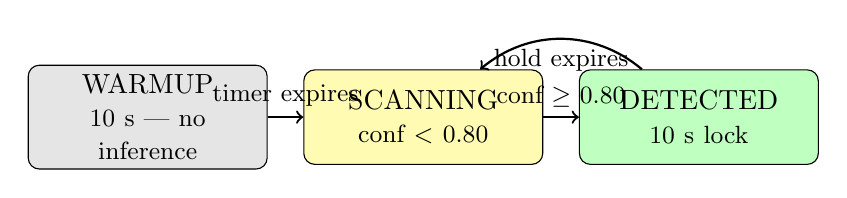
\begin{tikzpicture}[node distance=3.5cm, auto,
      state/.style={rectangle, rounded corners, draw, fill=blue!10,
                    text width=2.8cm, align=center, minimum height=1.2cm}]
      \node[state, fill=gray!20] (warmup)  {WARMUP\\{\small 10 s — no inference}};
      \node[state, fill=yellow!30, right of=warmup] (scan) {SCANNING\\{\small conf $<$ 0.80}};
      \node[state, fill=green!25, right of=scan]  (det)  {DETECTED\\{\small 10 s lock}};

      \draw[->, thick] (warmup) -- node[above]{\small timer expires} (scan);
      \draw[->, thick] (scan)   -- node[above]{\small conf $\geq$ 0.80} (det);
      \draw[->, thick] (det) to[bend right=40] node[below]{\small hold expires} (scan);
    \end{tikzpicture}
  \end{center}
  \vspace{0.2cm}
  \begin{columns}
    \column{0.32\textwidth}
      \textbf{\textcolor{gray}{Warmup (grey overlay)}}
      \begin{itemize}
        \item Camera starts immediately
        \item No inference for 10 s
        \item Shows ``No leaf detected''
        \item Lets sensor settle
      \end{itemize}
    \column{0.32\textwidth}
      \textbf{\textcolor{olive}{Scanning (grey overlay)}}
      \begin{itemize}
        \item Inference every frame
        \item Shows ``No leaf detected''
        \item Waits for confident hit
      \end{itemize}
    \column{0.32\textwidth}
      \textbf{\textcolor{leafgreen}{Detected (coloured overlay)}}
      \begin{itemize}
        \item Locks result for 10 s
        \item No new results accepted
        \item Green = healthy
        \item Red = disease
        \item Countdown shown
      \end{itemize}
  \end{columns}
\end{frame}

% ─────────────────────────────────────────────────────────────────────────────
\section{Challenges}

\begin{frame}{Challenges Faced}
  \begin{tabular}{p{4.5cm} p{7cm}}
    \toprule
    \textbf{Challenge} & \textbf{How it was resolved} \\
    \midrule
    TF/Keras 3 incompatible with Python 3.12 &
      Migrated entire pipeline to PyTorch + ONNX Runtime \\[4pt]
    \texttt{onnxscript} missing on Pi &
      Used legacy ONNX exporter (\texttt{dynamo=False, opset=17}) \\[4pt]
    INT8 calibration broken — 20\% accuracy &
      \texttt{quant\_pre\_process} renames input tensor; read actual name dynamically from model graph \\[4pt]
    QDQ format breaks Hardswish &
      Switched to \texttt{QuantFormat.QOperator} \\[4pt]
    \texttt{picamera2} absent in venv &
      Recreated venv with \texttt{--system-site-packages} \\[4pt]
    \texttt{cv2.imshow} fails over SSH &
      Set \texttt{export DISPLAY=:0} \\[4pt]
    Model collapsed to Corn\_healthy &
      Corn (monocot) visually incompatible with Tomato/Potato/Pepper (dicot); removed from training \\[4pt]
    Class imbalance $\Rightarrow$ Late blight bias &
      Added balanced mode with 1,000 images/class hard cap \\
    \bottomrule
  \end{tabular}
\end{frame}

% ─────────────────────────────────────────────────────────────────────────────
\section{Results \& Conclusion}

\begin{frame}{Results Summary}
  \begin{columns}
    \column{0.48\textwidth}
      \textbf{Model performance}
      \begin{center}
      \begin{tabular}{lcc}
        \toprule
         & float32 & INT8 \\
        \midrule
        Size      & 3.8 MB  & \textbf{1.1 MB} \\
        Latency   & 17.3 ms & \textbf{6.1 ms} \\
        Acc.\ drop & —      & $<$2\% \\
        \bottomrule
      \end{tabular}
      \end{center}
      \vspace{0.3cm}
      \textbf{Confusion matrix}
      \begin{center}
        
\includegraphics[width=0.85\linewidth]{confusion_matrix.png}
      \end{center}
    \column{0.48\textwidth}
      \textbf{Targets vs.\ achieved}
      \begin{center}
      \begin{tabular}{lcc}
        \toprule
        Target & Goal & Result \\
        \midrule
        Latency  & $<$1500 ms & \textcolor{leafgreen}{\textbf{6.1 ms}} \\
        Size     & $<$10 MB   & \textcolor{leafgreen}{\textbf{1.1 MB}} \\
        Acc.\ drop & $<$2\%   & \textcolor{leafgreen}{\textbf{$<$2\%}} \\
        Offline  & Yes        & \textcolor{leafgreen}{\textbf{Yes}} \\
        \bottomrule
      \end{tabular}
      \end{center}
      \vspace{0.3cm}
      \begin{block}{All targets met}
        The INT8 model runs \textbf{246$\times$ under} the latency budget, fits in 1.1 MB, and runs entirely offline on the Pi 5.
      \end{block}
  \end{columns}
\end{frame}

\begin{frame}{Conclusion \& Future Work}
  \begin{columns}
    \column{0.48\textwidth}
      \textbf{What we built}
      \begin{itemize}
        \item End-to-end offline plant disease detector on Raspberry Pi 5
        \item MobileNetV3-Small, two-stage fine-tuned on 15 classes
        \item INT8 ONNX model: 1.1 MB, 6 ms inference
        \item Live camera with detection state machine, confidence gating, and 10 s hold lock
      \end{itemize}
    \column{0.48\textwidth}
      \textbf{Future work}
      \begin{itemize}
        \item Fine-tune on real field photos (lab $\rightarrow$ field gap)
        \item Text-to-speech output for low-literacy users
        \item Expand to Grape, Apple, Rice classes
        \item Quantization-aware training (QAT) for lower accuracy drop
        \item Lightweight Android companion app via Bluetooth
        \item Solar-powered enclosure for full field deployment
      \end{itemize}
  \end{columns}
  \vspace{0.5cm}
  \begin{center}
    \large\textbf{GitHub:} \texttt{github.com/vanshdhar999/EdgeAI-Project}
  \end{center}
\end{frame}

% ─────────────────────────────────────────────────────────────────────────────
\begin{frame}
  \begin{center}
    \vspace{1cm}
    {\Huge \textbf{Thank You}}\\[0.8cm]
    {\large Aayush Jeevan Patil (22220) \quad · \quad Vansh Dhar (22156)}\\[0.4cm]
    {\normalsize \texttt{github.com/vanshdhar999/EdgeAI-Project}}
  \end{center}
\end{frame}

\end{document}
